% Built on the VLDB template (acmart with pvldb.sty), as the Hermes and OntoDB papers are.

\documentclass[sigconf, nonacm]{acmart}

\usepackage{pvldb}
% Packages and macros, following the conventions of the KROMA, MOIRA, and Hermes papers.
\usepackage{amsmath}
\usepackage{amssymb}
\usepackage{booktabs}
\usepackage{multirow}
\usepackage{xcolor}
\usepackage{colortbl}
\definecolor{ours}{HTML}{DCEBFA}  % light blue: where OntoDB is best
\usepackage{xspace}
\usepackage{balance}
\usepackage{pgfplots}
\usepackage[ruled,linesnumbered,noend]{algorithm2e}
\pgfplotsset{compat=1.17}
\usetikzlibrary{positioning,arrows.meta}

% Long identifiers must not overflow the narrow columns.
\setlength{\emergencystretch}{2em}

% Tight layout, as in the MOIRA and Hermes papers: no stretched columns, small caption gaps,
% compact lists and floats. (acmart forbids titlesec.)
\raggedbottom
\usepackage[skip=0.5ex]{caption}
\setlength{\abovecaptionskip}{3pt}
\setlength{\belowcaptionskip}{3pt}
\usepackage{enumitem}
\setlist{nosep, leftmargin=*}
\setlength{\textfloatsep}{8pt plus 2pt minus 2pt}
\setlength{\floatsep}{6pt plus 2pt minus 2pt}
\setlength{\intextsep}{6pt plus 2pt minus 2pt}
\setlength{\dbltextfloatsep}{8pt plus 2pt minus 2pt}

\newcommand{\sys}{\textsc{OntoDB}\xspace}
\newcommand{\sparql}{SPARQL\xspace}
\newcommand{\kw}[1]{{\ensuremath{\mathsf{#1}}}\xspace}
\newcommand{\stitle}[1]{\vspace{1.2ex}\noindent{\bf #1}}
\newcommand{\ie}{\emph{i.e.,}\xspace}
\newcommand{\eg}{\emph{e.g.,}\xspace}
\newcommand{\desc}{\mathrm{desc}}
\newcommand{\po}{\mathit{po}}
\newcommand{\lo}{\mathit{lo}}
\newcommand{\ef}{\mathit{ef}}


\renewcommand\vldbdoi{XX.XX/XXX.XX}
\renewcommand\vldbpages{XXX-XXX}
\renewcommand\vldbavailabilityurl{https://github.com/lamng3/OntoDB}

\begin{document}

\title{Meaning Under a Class: Hierarchy-Filtered\\Vector Search Inside an Ontology Store}

\author{Lam Nguyen}
\affiliation{%
  \institution{Case Western Reserve University}
  \city{Cleveland}
  \state{Ohio}
  \country{USA}
}
\email{ltn18@case.edu}

\begin{abstract}
Ontologies pair a class hierarchy with names that embeddings can compare, and a
natural question combines the two: which terms are closest in meaning to a given
term \emph{and lie under a given class}?
Vector databases answer it by passing the index a filter, and approximate indexes
silently lose recall when the filter is selective: on four ontologies, FAISS
indexes asked for the ten nearest terms under a class return on average 61\% (IVF)
and 64\% (HNSW) of the right answers, and 2\% (HNSW) for a query that lies outside a
small class; a 16 times larger beam raises that to only 20\%.
This paper presents a vector search that lives inside an ontology store and uses
the hierarchy as the filter.
(1) We prove that no linear order of points keeps nearest neighbors close, and
measure how few a sorted index of an ontology puts within a short scan.
(2) We label the class hierarchy with postorder intervals in the store's own
B+ tree, so that a class's members are a few range scans and membership is a
binary search, and we store IVF posting lists as key ranges of the same tree.
(3) We show that in an ontology the class filter is correlated with the vectors, so
the independence assumption behind filtered-search costing fails, and give
four filtering strategies, a cost model for the crossover between resolving the
class and testing it per row, and a rule that picks between them.
(4) We evaluate against FAISS, hnswlib, and DuckDB on the Gene Ontology, the Human
Phenotype Ontology, Uberon, and ChEBI (218,723 terms), with queries that are
stored terms and queries that are not.
Across 958 queries our rule returns recall 0.999 and never falls below 0.99, with a
median of 26\,$\mu$s; for classes of at most ten members it is 33 times faster than
an exact FAISS scan with an ID selector (2.1 against 70\,$\mu$s).
\end{abstract}


\keywords{ontology, vector search, filtered nearest neighbor search, class hierarchy, B+ tree}

\maketitle

\vldbtopmatter

\section{Introduction}
\label{sec-intro}

An ontology is a class hierarchy whose classes have names, and names can be
embedded: the Gene Ontology, the Human Phenotype Ontology, and ChEBI each give tens
or hundreds of thousands of terms a vector, so that terms close in meaning are close
in cosine similarity.
Tasks such as ontology matching, term normalization, and retrieval over annotated
data then ask for \emph{the terms nearest to a given term that lie under a given
class}: the nearest phenotype to ``short stature'' under ``abnormality of the
skeletal system'', the nearest process to ``apoptotic process'' under ``cell
death''.
The hierarchy defines the filter, and the vectors rank what passes it.

Vector databases answer such queries by giving the index a predicate, and they leave
four problems open.
\textbf{C1. A sorted index does not hold meaning.}
Triple stores answer patterns with range scans over sorted permutations, and it is
tempting to believe that terms close in meaning are close in the order, so that a
scan could serve similarity.
No linear order can keep all neighbors close (Section~\ref{sec-order}), and on four
ontologies the best order we tried finds 38\% to 56\% of a term's ten nearest
neighbors within 100 positions.
\textbf{C2. Filtered approximate search loses recall without warning.}
An IVF or graph index with a filter probes the lists or the walk nearest the query;
when few of the terms there pass the filter, it returns fewer, worse answers and
reports no error.
On our workload FAISS indexes with an ID selector return recall 0.61 (IVF) and 0.64
(HNSW), and 0.02 for HNSW when the query lies outside a small class.
\textbf{C3. The filter is correlated with the vectors.}
Filtered search is costed by assuming the filter is independent of the similarity,
so that $k/f$ candidates suffice for a filter that passes a fraction $f$.
In an ontology the neighbors of a term lie under the term's own ancestors, so the
estimate is wrong in both directions (Section~\ref{sec-filter}).
\textbf{C4. The filter lives in another system.}
A vector database knows nothing of the hierarchy: the caller must resolve a class to
its members, keep a table of them, and keep it current.

\begin{example}
\label{exa-motivation}
Let $q$ be \emph{apoptotic process} and $c$ the class \emph{cell death} in the Gene
Ontology.
A vector index returns neighbors from anywhere in the ontology, and a post-filter
keeps those under $c$ only if enough of them are.
For a query from outside a class of at most ten members, an ID-selector IVF returns
on average 5\% of the right answers.
Here the engine finds the 97 members of $c$ with one range scan of the B+ tree that
holds the triples, scores them exactly, and returns \emph{apoptotic process involved
in development} (cosine 0.865) first, in under a millisecond in a web page.
\end{example}

\stitle{Contributions}.
We build the filter into the store.
\begin{enumerate}
\item \textbf{A bound and a measurement on order} (Section~\ref{sec-order}): every
  linear order of a graph's vertices separates some edge by $(N{-}1)/D$ positions,
  and on four ontologies no order of the terms holds more than 56\% of the ten
  nearest neighbors within 100 positions.
\item \textbf{The hierarchy as a membership test} (Section~\ref{sec-filter}):
  postorder intervals in the engine's B+ tree make a class's members a few range
  scans and membership a binary search, which lets a vector search test the filter
  per row without resolving it.
\item \textbf{A filtering rule that does not lose recall} (Section~\ref{sec-filter}):
  four strategies, a measurement that the class filter is correlated with the
  vectors, a cost model for the crossover between resolving the class and testing
  it, and a rule that picks between them and is exact for the classes where
  approximate indexes fail.
\item \textbf{Vector indexes whose lists live in the triple tree}
  (Section~\ref{sec-index}): IVF posting lists stored as key ranges of the same
  B+ tree, so that they page, cache, and latch with the triples.
\end{enumerate}
We evaluate against FAISS, hnswlib, and DuckDB on four ontologies, with queries that are
stored terms and queries that are not (Section~\ref{sec-exp}).
The code, data scripts, and benchmark programs are at the artifact URL above.

\section{Preliminaries}
\label{sec-pre}

\begin{table}[t]
\caption{Notation.}
\label{tab-notation}
\small
\begin{tabular}{@{}p{2.1cm}p{5.65cm}@{}}
\toprule
Symbol & Meaning \\
\midrule
$H=(\mathcal{C},E)$ & the class hierarchy, a DAG of classes and subclass edges \\
$\desc(c)$ & the classes at or below $c$, including $c$ \\
$\po(c)$, $\lo(c)$ & postorder number of $c$; smallest number in its subtree of the spanning forest \\
$I(c)$ & the set of intervals that covers the numbers of $\desc(c)$ \\
$f(c)$ & fraction of terms below $c$: $|\desc(c)|/N$ \\
$N$, $d$ & number of terms with vectors; vector dimension \\
$\mathbf{v}(t)$, $\mathrm{sim}$ & unit vector of term $t$; cosine similarity \\
$q$, $k$ & the query vector; the number of neighbors asked for \\
$\mathrm{near}(q,c,k)$ & the $k$ terms of $\desc(c)$ nearest to $q$ \\
$\nu$, $\rho$ & IVF: number of lists; lists probed per query \\
$M$, $\ef$ & HNSW: links per node; search beam width \\
$G$, $D$ & a graph and its diameter \\
$\gamma_m$, $\gamma_h$ & cost per member of resolving a class; cost of a masked walk \\
$\theta$ & the auto rule's threshold on $|\desc(c)|$ \\
\bottomrule
\end{tabular}
\end{table}

\stitle{Terms, classes, vectors}.
An ontology has classes $\mathcal{C}$ related by \texttt{rdfs:subClassOf} edges $E$,
forming a directed graph $H$ in which cycles are collapsed (classes on a cycle are
equivalent).
We write $\desc(c)$ for the classes at or below $c$, including $c$.
Each of $N$ terms, here the classes of the ontology, has a name, and an embedding model
maps the name to a unit vector $\mathbf{v}(t)\in\mathbb{R}^d$; the similarity of two
terms is the cosine $\mathbf{v}(t)\cdot\mathbf{v}(u)$.

\begin{definition}[Hierarchy-filtered nearest neighbors]
\label{def-near}
For a query vector $q$, a class $c$, and $k\ge 1$, $\mathrm{near}(q,c,k)$ is the
set of $k$ terms $t\in\desc(c)$ with the largest $q\cdot\mathbf{v}(t)$.
\end{definition}

\noindent
The query vector is the embedding of a stored term, as in ontology matching between
two parts of one ontology, or of text that is not a term, such as a synonym or a word
from a document.
A term used as the query is never its own neighbor.
An answer $A$ is judged by its \emph{recall}, $|A\cap\mathrm{near}(q,c,k)|/k$, against
exact search over $\desc(c)$.
A system that returns fewer than $k$ answers has a recall below one.

\stitle{The store}.
The vectors live in an ontology store, OntoDB~\cite{ontodb}, that keeps triples in three
B+ trees behind a buffer pool and keeps the hierarchy as labels in the same engine.
This paper uses three of its parts: the B+ tree and its range scan, the postorder
labelling of the hierarchy (Section~\ref{sec-filter}), and the buffer pool that pages
all of it.

\section{Order Is Not Similarity}
\label{sec-order}

A triple store answers a bound prefix with one range scan over a sorted index, and it
is tempting to hope that terms close in meaning are close in the order, so that a scan
of a window could serve a similarity query.

\begin{lemma}[Bandwidth]\label{lem-bw}
Let $G$ be a graph with $N$ vertices and diameter $D$.
In every linear order of the vertices some edge joins vertices at least $(N-1)/D$
positions apart.
\end{lemma}

\noindent
The first and last vertices of an order are $N-1$ apart and joined by a path of at
most $D$ edges, so some edge of the path covers at least $(N-1)/D$ positions
(Appendix~\ref{apx-proofs}).
For the neighbor graph of a $d$-dimensional grid of $N=g^d$ points (diameter
$d(g-1)$) that is at least $g^{d-1}/d$ positions in any order, so a scan of width $w$
cannot hold all neighbors unless $w$ is that large.
Space-filling curves keep neighbors close on average and need several scans to cover
a query ball; they do not escape the lemma.

\stitle{What real orders give}.
We embedded the term names of four ontologies (Section~\ref{sec-exp}) and, for 2,000
random terms, took the ten nearest by cosine.
Table~\ref{tab-order} gives the share of those neighbors found within $\pm100$
positions of the term in each order: the hierarchy's postorder, the dictionary's
first-seen ids (an engine's default order), the alphabetical order of the names, and a
random order.

\begin{table}[t]
\caption{Share of a term's ten nearest neighbors (cosine) found within $\pm$100 positions, and the median position gap to the nearest neighbor, by order of the terms. 2,000 queries.}
\label{tab-order}
\small
\resizebox{\columnwidth}{!}{%
\begin{tabular}{@{}lrrrrrrrr@{}}
\toprule
 & & \multicolumn{4}{c}{share within $\pm$100} & \multicolumn{3}{c}{median gap} \\
\cmidrule(lr){3-6}\cmidrule(lr){7-9}
Ontology & terms & hierarchy & first-seen id & alphabetical & random & hierarchy & id & random \\
\midrule
GO & 38,092 & \textbf{0.38} & 0.21 & 0.33 & 0.005 & 45 & 1,739 & 10,823 \\
HPO & 19,894 & \textbf{0.56} & 0.23 & 0.28 & 0.009 & 6 & 2,033 & 5,589 \\
Uberon & 15,047 & \textbf{0.39} & 0.23 & 0.35 & 0.013 & 41 & 930 & 4,374 \\
ChEBI & 218,723 & 0.23 & 0.13 & \textbf{0.41} & 0.001 & 444 & 4,351 & 61,743 \\
\bottomrule
\end{tabular}}
\end{table}


\noindent
Three things follow.
First, no order is enough: the best finds 38\% to 56\% of the neighbors in a window
of 200 positions, a window that is 0.1\% to 1.3\% of the ontology.
Second, which order is best depends on the ontology: the hierarchy's postorder wins on
three, and alphabetical order wins on ChEBI, whose names share prefixes
(``\emph{N}-acetyl-\ldots''); what the hierarchy supplies is \emph{structure}, not
similarity.
Third, first-seen ids carry some locality (0.13 to 0.23) that comes from the file the
ontology was loaded from and not from the engine.
The order is therefore useful for the hierarchy and is no substitute for a vector index.

\section{Filtering by a Class}
\label{sec-filter}

\stitle{The hierarchy as a membership test}.
Collapse each cycle of $H$ into one class, pick for every class with several parents the
parent with the longest path from a root, and number the classes in postorder of the
resulting spanning forest.
In a forest the classes below $c$ are those whose number lies in one interval
$[\lo(c),\po(c)]$; in a DAG each class carries a \emph{set} of intervals $I(c)$, built
children first by merging its own interval with the sets of its children
(Agrawal et al.~\cite{agrawal1989}), and $|I(c)|\le 1+|E'(c)|$ for the $|E'(c)|$
non-tree edges below $c$.
The numbers are keys of the engine's B+ tree, $(\po(c),c,0)$ for each class, so
\begin{itemize}
\item the \emph{members} of $c$ are one range scan per interval of $I(c)$, in
  $O(|I(c)|)$ descents plus the members, and
\item whether a class $u$ lies below $c$ is a binary search of $\po(u)$ in $I(c)$, with
  no scan and no memory beyond the intervals.
\end{itemize}
On the four ontologies the mean class needs 1.3 to 2.0 intervals (at most 4,329, within the
bound), against 5.3 million ancestor pairs for ChEBI's closure and 402,305 intervals.
The labels are built in 4 to 69\,ms for 13,850 to 218,723 classes and rebuilt when the
hierarchy changes; term ids are untouched.

\stitle{Four strategies}.
A query $\mathrm{near}(q,c,k)$ can be answered in four ways, all returning terms of
$\desc(c)$ only.
\begin{description}
\item[Pre-filter] resolves $c$ to its members by range scans and scores them exactly:
  about $\gamma_m\,|\desc(c)|$ time, where $\gamma_m$ covers a scan step, a lookup from
  term to row, and one dot product.
\item[Post-filter] asks an index for $k'>k$ answers, keeps those below $c$ (a binary
  search each), and multiplies $k'$ by four until $k$ remain or the index is exhausted.
\item[Masked search] hands the index the predicate ``the row's number lies in an
  interval of $I(c)$'', so a list scan or a graph walk skips rows outside $c$ and
  nothing is resolved in advance; each row touched costs one binary search.
  Masked IVF keeps probing lists, nearest first, until it holds $k$ allowed rows or
  has probed all (Algorithm~\ref{alg-ivf}); masked HNSW still crosses rows it may not
  return, to keep the graph connected, and keeps a beam of $\ef$ allowed candidates.
\item[Auto] pre-filters when $|\desc(c)|\le\theta$ and otherwise runs masked HNSW.
\end{description}

\begin{algorithm}[t]
\caption{\textsc{Near}$(q,c,k)$: the auto rule}\label{alg-auto}
\small
\lIf{$c$ is not a class of $H$}{\Return $\emptyset$}
\eIf{$|\desc(c)|\le\theta$}{
  $R \gets$ the rows of the keys in the range scans $[(a,0,0),(b{+}1,0,0))$ for each $[a,b]\in I(c)$\;
  \Return the $k$ rows of $R$ with the largest $q\cdot\mathbf{v}$ \tcp*{pre-filter: exact}
}{
  \Return \textsc{MaskedHnsw}$(q,k,\ef,\;r\mapsto \po(r)\in I(c))$\;
}
\end{algorithm}

\begin{algorithm}[t]
\caption{\textsc{MaskedHnsw}$(q,k,\ef,\mathit{allowed})$}\label{alg-hnsw}
\small
descend the upper layers greedily from the entry point to the node nearest $q$ (the filter is not applied)\;
$\mathit{frontier} \gets \{$that node$\}$; $W \gets \emptyset$ \tcp*{$W$ holds allowed rows only}
\While{$\mathit{frontier}\ne\emptyset$}{
  $x \gets$ the frontier node nearest $q$\;
  \lIf{$|W|\ge\ef$ and $x$ is farther than the worst row of $W$}{\textbf{break}}
  \For{each unvisited neighbor $y$ of $x$ on layer 0}{
    add $y$ to $\mathit{frontier}$ whether or not it is allowed\;
    \lIf{$\mathit{allowed}(y)$}{add $y$ to $W$; drop the worst row if $|W|>\ef$}
  }
}
\Return the $k$ best rows of $W$\;
\end{algorithm}

\begin{algorithm}[t]
\caption{Masked IVF: the $k$ best rows allowed by the class}\label{alg-ivf}
\small
sort the $\nu$ lists by the similarity of their centroids to $q$\;
$\mathit{best} \gets \emptyset$; $\mathit{seen} \gets 0$\;
\For{each list $\ell$ in that order}{
  \For{each key $(\ell,r,0)$ of the prefix scan of $\ell$ in the B+ tree}{
    \lIf{the number of row $r$ lies in an interval of $I(c)$}{score $r$; keep it among the $k$ best}
  }
  $\mathit{seen} \gets \mathit{seen}+1$\;
  \lIf{$\mathit{seen}\ge\rho$ and $|\mathit{best}|=k$}{\textbf{break}}
}
\Return $\mathit{best}$\;
\end{algorithm}

\begin{lemma}[Exactness and completeness]\label{lem-exact}
Pre-filter returns exactly $\mathrm{near}(q,c,k)$. Masked IVF returns
$\min(k,|\desc(c)|)$ answers, and exactly $\mathrm{near}(q,c,k)$ when $\rho=\nu$.
\end{lemma}

\noindent
Pre-filter scores every member; masked IVF stops only with $k$ allowed rows or after
all lists, and with all lists probed it has scored every allowed row
(Appendix~\ref{apx-proofs}).
Masked HNSW (Algorithm~\ref{alg-hnsw}) crosses disallowed nodes to keep the graph
connected and keeps a beam of $\ef$ \emph{allowed} rows, so it does not stop early for
lack of allowed neighbors, which is also why it is slow for a small class: it walks until
it has found $\ef$ of them.
An index asked for $k$ answers and filtered afterwards has neither property.

\stitle{The filter is correlated with the vectors}.
Costing a filtered search by the filter's selectivity assumes independence: a filter
that passes a fraction $f(c)$ of the terms needs about $k/f(c)$ candidates.
In an ontology the names of a class's descendants resemble the class and one
another, so the neighbors of a term concentrate under the term's own ancestors.
Table~\ref{tab-correlation} measures it: for a query that is a member of $c$, or a synonym
of one, the share of the unfiltered top 100 under $c$ is 0.03 to 0.59, which is 10 to 100
times the fraction of terms below $c$ for classes of up to 1,000 members, and for a
query outside it falls to 0.00 to 0.24, below that fraction for the largest classes.
The estimate $k/f(c)$ is therefore too large for an inside query, which a post-filter
answers cheaply, and too small for an outside one, for which a post-filter's
candidates run out before $k$ allowed rows are seen.

\begin{table}[t]
\caption{Share of a query's unfiltered top 100 neighbors that lie under the class, by query kind and number of classes below $c$ (pooled mean; the independence estimate would be the fraction of terms below $c$).}
\label{tab-correlation}
\small
\begin{tabular}{@{}lrrrr@{}}
\toprule
Below $c$ & independent & inside & outside & synonym \\
\midrule
$\le$10 & 0.000 & 0.03 & 0.00 & 0.03 \\
11--100 & 0.001 & 0.14 & 0.00 & 0.11 \\
101--1,000 & 0.012 & 0.31 & 0.01 & 0.29 \\
1,001--5,000 & 0.054 & 0.54 & 0.03 & 0.43 \\
$>$5,000 & 0.334 & 0.59 & 0.24 & 0.46 \\
\bottomrule
\end{tabular}
\end{table}


\stitle{Resolve or test}.
Masked search can test the filter per row (one binary search over $I(c)$) or resolve it
first into a bitmap by range scans.
Resolving costs $\gamma_m|\desc(c)|$ whether or not the search ever looks at those
rows; testing costs only for rows the walk touches.
Pre-filtering resolves and scores, so it is the right plan exactly when
$\gamma_m|\desc(c)|$ is less than the masked walk's cost $\gamma_h$:
\[
\mathrm{pre\text{-}filter\ wins} \iff |\desc(c)| < \theta = \gamma_h/\gamma_m .
\]
The walk's cost depends on where the query is: for a query inside $c$ the walk finds
allowed rows at once, and for one outside it must cross rows it cannot return, so
$\gamma_h$ and $\theta$ differ, and a single threshold has to sit between them
(Section~\ref{sec-exp}).

\section{Vector Indexes in the Store}
\label{sec-index}

The engine keeps one unit vector per term in memory, loaded from a checksummed file
whose records name terms by spelling, so a file survives a dictionary that numbers
terms differently.
Embeddings come from outside; the engine stores and searches them with four index
families, each a different trade between exactness, memory, and build time.

\stitle{Flat}.
Score every vector with eight independent accumulators (a plain loop is not
vectorized by the compiler without fast-math and made our first exact baseline four
times too slow): $O(Nd)$ and exact.

\stitle{IVF with lists in the triple tree}.
Spherical $k$-means with $k$-means++ seeding~\cite{arthur2007} gives $\nu=2.6\sqrt{N}$
centroids, each vector goes to its nearest, and a query scores the centroids and
reads the $\rho$ nearest lists, for a cost $\nu d+\rho (N/\nu) d$.
The design choice is where the lists live: as key ranges of the B+ tree that holds the
triples.
The pair (list, row) is a key $(\mathrm{list},\mathrm{row},0)$, so a list is a prefix
scan, and the lists page, cache, and latch like every other index of the engine, with
the buffer pool, the page latches, and the checksums already there; a separate vector
library would add its own memory and its own copy of the data.
The price is a 24-byte key per row and a random read of the vector per entry, which
Section~\ref{sec-exp} measures against a contiguous list.

\stitle{HNSW}.
The layered proximity graph of Malkov and Yashunin~\cite{malkov2020} with the paper's
neighbor-selection heuristic, $M{=}16$ links (32 on layer 0), and construction beam
200; search takes an optional row filter and still crosses rows it may not return.

\stitle{In the engine}.
The indexes are driven from the shell and from the browser build.
After loading the ontology and its vectors and building the labels and the indexes,
\begin{small}\begin{verbatim}
\hindex build
\vload go.ovec
\vindex build all
\similar "apoptotic process" 4 under "cell death"
\end{verbatim}\end{small}
prints the neighbors with their cosine, the strategy the rule chose, and the time
(here for an 834-class slice of the Gene Ontology in a browser):
\begin{small}\begin{verbatim}
0.865  apoptotic process involved in development
0.802  apoptotic process involved in morphogenesis
0.786  epithelial cell apoptotic process
0.779  neuron apoptotic process     [pre-filter, 0.8 ms]
\end{verbatim}\end{small}
Forcing a strategy (\texttt{using post-ivf}, \texttt{using mask-hnsw}) runs the others.

\stitle{Product quantization}.
Cutting a vector into $m$ pieces and replacing each by its nearest of 256 learned
centers~\cite{jegou2011} gives $m$ bytes per vector, scored through $m$ tables of 256
dot products; it is for memory, not speed, at this size, and we do not use it in the
filtered experiments.

\section{Experimental Study}
\label{sec-exp}

We evaluate the filtered search along four research questions.
\begin{itemize}
\item \textbf{[RQ1] Order}: how much of a term's neighborhood does a sorted order of an
  ontology hold? (Table~\ref{tab-order}, Section~\ref{sec-order}.)
\item \textbf{[RQ2] Filtered search}: what do the strategies return and cost, against
  FAISS filtering with ID selectors?
\item \textbf{[RQ3] The rule}: is the class filter correlated with the vectors, does testing
  it per row beat resolving it, and where is the crossover?
\item \textbf{[RQ4] The indexes}: what do IVF with lists in the triple tree and HNSW cost
  against FAISS and hnswlib, and does the design scale to 218,723 terms?
\end{itemize}

\stitle{Setup}.
The ontologies are the Gene Ontology~\cite{ashburner2000} (38,092 terms, release
2026-07-26 without obsolete terms), the Human Phenotype Ontology~\cite{kohler2021}
(19,894), Uberon~\cite{mungall2012} (15,047), and ChEBI~\cite{hastings2016} (218,723),
each with the \texttt{is\_a} edges as the hierarchy and the term names embedded by
\texttt{all-MiniLM-L6-v2}~\cite{reimers2019} into 384 dimensions on a CPU.
For each ontology and each of five sizes of $|\desc(c)|$ ($\le$10, 11--100, 101--1,000,
1,001--5,000, $>$5,000) we draw up to 20 classes that have subclasses, and for each class
three queries: a stored term inside the class, one outside it, and the embedding of a
synonym of a stored member (5,000 synonyms sampled per ontology), which is not a stored
vector.
Answers are scored against exact search over the class's members, with the query term
excluded; there are 958 queries per strategy.
OntoDB uses IVF with $\nu=2.6\sqrt N$ lists and $\rho=16$, HNSW with $M{=}16$,
construction beam 200, and $\ef{=}64$, and the auto rule with $\theta=4{,}096$; FAISS
1.15.1 uses \texttt{IndexFlatIP}, \texttt{IndexIVFFlat} (same $\nu$, nprobe 16), and
\texttt{IndexHNSWFlat} (same $M$, efSearch 64), each searched with an
\texttt{IDSelectorBitmap} of the class's members; hnswlib 0.8.0 appears in the unfiltered
comparison.
The members of a class for FAISS come from a descendant table built outside the timer,
which favors FAISS.
Every time is the mean of three runs after one warm-up, on one thread of an Apple M2 Pro
with 16\,GiB; FAISS is called once per query from Python, and its call overhead (about
10\,$\mu$s) is included.

\subsection{RQ2: Filtered Search}

\begin{table*}[t]
\caption{Ten nearest terms under a class: recall@10 / microseconds per query, by number of classes below $c$ and by query kind, pooled over 4 ontologies. FAISS runs each query with an ID selector of the class's members (their lookup is not timed). Bold marks the fastest strategy with recall at least 0.99; blue marks \sys{}.}
\label{tab-filtered}
\small
\begin{tabular}{@{}llccccccc@{}}
\toprule
Below $c$ & query & DuckDB join & FAISS exact & FAISS IVF & FAISS HNSW & pre-filter & masked HNSW & auto \\
\midrule
$\le$10 & inside $c$ & 1.00 / 718 & 1.00 / 71 & 0.79 / 29 & 0.87 / 50 & \cellcolor{ours}\textbf{1.00 / 2.1} & 1.00 / 42.1\,k & 1.00 / 2.2 \\
11--100 &  & 1.00 / 811 & 1.00 / 72 & 0.82 / 30 & 0.85 / 49 & \cellcolor{ours}\textbf{1.00 / 7.9} & 1.00 / 37.4\,k & 1.00 / 8.1 \\
101--1,000 &  & 1.00 / 1.2\,k & 1.00 / 90 & 0.89 / 35 & 0.91 / 50 & \cellcolor{ours}\textbf{1.00 / 47} & 1.00 / 5.9\,k & 1.00 / 49 \\
1,001--5,000 &  & 1.00 / 2.6\,k & \textbf{1.00 / 213} & 0.93 / 46 & 0.98 / 47 & 1.00 / 244 & 1.00 / 1.2\,k & 1.00 / 396 \\
$>$5,000 &  & 1.00 / 28.6\,k & 1.00 / 2.0\,k & 0.93 / 81 & 0.98 / 56 & 1.00 / 4.9\,k & 1.00 / 506 & \cellcolor{ours}\textbf{1.00 / 456} \\
\midrule
$\le$10 & outside $c$ & 1.00 / 708 & 1.00 / 69 & 0.05 / 29 & 0.02 / 51 & \cellcolor{ours}\textbf{1.00 / 2.1} & 1.00 / 42.2\,k & 1.00 / 2.2 \\
11--100 &  & 1.00 / 802 & 1.00 / 71 & 0.06 / 29 & 0.04 / 49 & \cellcolor{ours}\textbf{1.00 / 7.8} & 1.00 / 38.8\,k & 1.00 / 8.3 \\
101--1,000 &  & 1.00 / 1.1\,k & 1.00 / 88 & 0.23 / 29 & 0.24 / 50 & \cellcolor{ours}\textbf{1.00 / 47} & 1.00 / 18.2\,k & 1.00 / 51 \\
1,001--5,000 &  & 1.00 / 2.6\,k & \textbf{1.00 / 205} & 0.40 / 33 & 0.39 / 49 & 1.00 / 245 & 1.00 / 9.3\,k & 1.00 / 652 \\
$>$5,000 &  & 1.00 / 27.4\,k & 1.00 / 2.0\,k & 0.58 / 61 & 0.73 / 62 & 1.00 / 5.0\,k & 0.99 / 1.9\,k & \cellcolor{ours}\textbf{0.99 / 1.9\,k} \\
\midrule
$\le$10 & synonym of a member & 1.00 / 708 & 1.00 / 49 & 0.74 / 25 & 0.76 / 48 & \cellcolor{ours}\textbf{1.00 / 2.2} & 1.00 / 25.3\,k & 1.00 / 2.3 \\
11--100 &  & 1.00 / 808 & 1.00 / 56 & 0.74 / 27 & 0.74 / 47 & \cellcolor{ours}\textbf{1.00 / 7.7} & 1.00 / 27.1\,k & 1.00 / 8.0 \\
101--1,000 &  & 1.00 / 1.1\,k & 1.00 / 87 & 0.82 / 33 & 0.88 / 51 & \cellcolor{ours}\textbf{1.00 / 47} & 1.00 / 8.9\,k & 1.00 / 50 \\
1,001--5,000 &  & 1.00 / 2.6\,k & \textbf{1.00 / 203} & 0.79 / 42 & 0.90 / 50 & 1.00 / 246 & 1.00 / 3.7\,k & 1.00 / 257 \\
$>$5,000 &  & 1.00 / 28.1\,k & \textbf{1.00 / 2.0\,k} & 0.88 / 75 & 0.91 / 59 & 1.00 / 5.1\,k & 0.98 / 615 & 0.98 / 596 \\
\bottomrule
\end{tabular}
\end{table*}


\stitle{Approximate indexes lose recall silently}.
Table~\ref{tab-filtered} and Figure~\ref{fig-recall} give the result.
Over the 958 queries FAISS's IVF and HNSW with an ID selector return recall 0.61 and 0.64,
and 59\% and 52\% of their queries are below 0.99.
The loss is worst where the filter is most selective and the query is far from it: for
a query outside a class of at most ten members they return 0.05 and 0.02.
A larger budget does not repair it (Table~\ref{tab-wide}): with half of all lists probed,
IVF reaches 0.52 for those queries at three times the time, and HNSW with a beam of 1,024
reaches 0.20 at 26 times the time, because the walk and the probed lists are the ones
near the query, where no member lives.
Over all queries the wide IVF reaches recall 0.91 in 204\,$\mu$s on average, the same time as
the rule, and 19\% of its queries are still below 0.99; the wide HNSW reaches 0.81 in 1.2\,ms.

\begin{figure}[t]
\centering
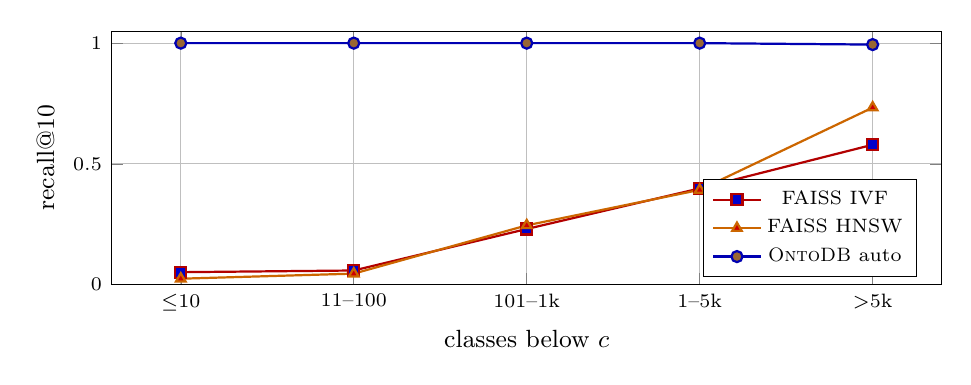
\begin{tikzpicture}
\begin{axis}[width=\columnwidth,height=4.8cm,symbolic x coords={<=10,11-100,101-1000,1001-5000,>5000},xtick=data,xticklabels={$\le$10,11--100,101--1k,1--5k,$>$5k},xlabel={classes below $c$},ylabel={recall@10},ymin=0,ymax=1.05,grid=both,legend pos=south east,legend style={font=\scriptsize},tick label style={font=\scriptsize},label style={font=\small}]
\addplot+[mark=square*,color=red!70!black,thick] coordinates {(<=10,0.051) (11-100,0.058) (101-1000,0.230) (1001-5000,0.398) (>5000,0.579)};
\addlegendentry{FAISS IVF}
\addplot+[mark=triangle*,color=orange!80!black,thick] coordinates {(<=10,0.024) (11-100,0.045) (101-1000,0.245) (1001-5000,0.392) (>5000,0.733)};
\addlegendentry{FAISS HNSW}
\addplot+[mark=*,color=blue!70!black,thick] coordinates {(<=10,1.000) (11-100,1.000) (101-1000,1.000) (1001-5000,1.000) (>5000,0.994)};
\addlegendentry{\sys{} auto}
\end{axis}
\end{tikzpicture}

\caption{Recall@10 for queries outside the class, by number of classes below it (pooled over the four ontologies).}
\label{fig-recall}
\end{figure}

\begin{table}[t]
\caption{FAISS with an ID selector at its default budget and at a much larger one (half of all IVF lists; HNSW beam 1,024): recall@10 / microseconds, queries outside the class, pooled.}
\label{tab-wide}
\small
\resizebox{\columnwidth}{!}{%
\begin{tabular}{@{}lrrrr@{}}
\toprule
Below $c$ & IVF & IVF, half the lists & HNSW & HNSW, beam 1,024 \\
\midrule
$\le$10 & 0.05 / 29 & 0.52 / 86 & 0.02 / 51 & 0.20 / 1.3\,k \\
11--100 & 0.06 / 29 & 0.68 / 88 & 0.04 / 49 & 0.35 / 1.2\,k \\
101--1,000 & 0.23 / 29 & 0.89 / 99 & 0.24 / 50 & 0.66 / 1.2\,k \\
1,001--5,000 & 0.40 / 33 & 0.97 / 160 & 0.39 / 49 & 0.78 / 1.2\,k \\
$>$5,000 & 0.58 / 61 & 0.99 / 1.1\,k & 0.73 / 62 & 0.95 / 1.5\,k \\
\bottomrule
\end{tabular}}
\end{table}


\stitle{Why}.
Table~\ref{tab-mechanism} shows the mechanism for IVF.
The lists an IVF index probes are the ones nearest the query, and the members of a small
class are somewhere else: for a query outside a class of at most ten members (four on
average), the 16 probed lists hold 0.2 of them, and outside a class of 11 to 100 (31 on
average) 1.1, where the answer needs ten.
For a query inside, they hold 3.5 of four and 19 of 31.
An index that cannot find allowed rows in the region it searches returns what it has,
and a filtered HNSW walk behaves the same way: it fills its beam with near nodes that are
not members.

\begin{table}[t]
\caption{Why an ID-selector IVF loses recall: the members of the class that lie in the 16 lists it probes, against the ten the answer needs (mean over the queries, pooled over the four ontologies).}
\label{tab-mechanism}
\small
\begin{tabular}{@{}lrrr@{}}
\toprule
Below $c$ & members & in probed lists, inside & outside \\
\midrule
$\le$10 & 4 & 3.5 & 0.2 \\
11--100 & 31 & 19.2 & 1.1 \\
101--1,000 & 308 & 120.8 & 12.6 \\
1,001--5,000 & 1,856 & 397.7 & 48.1 \\
$>$5,000 & 36,431 & 1,139.9 & 585.4 \\
\bottomrule
\end{tabular}
\end{table}


\begin{figure}[t]
\centering
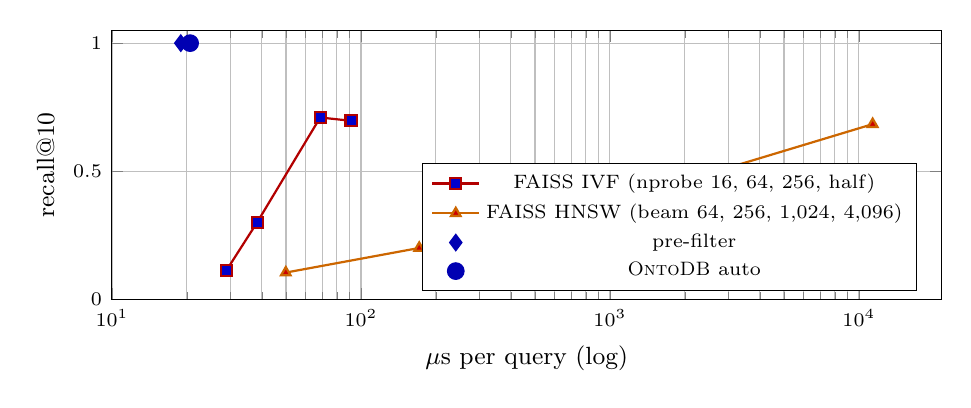
\begin{tikzpicture}
\begin{axis}[width=\columnwidth,height=5.0cm,xmode=log,xlabel={$\mu$s per query (log)},ylabel={recall@10},ymin=0,ymax=1.05,grid=both,legend pos=south east,legend style={font=\scriptsize},tick label style={font=\scriptsize},label style={font=\small}]
\addplot+[mark=square*,color=red!70!black,thick] coordinates {(28.8,0.113) (38.3,0.301) (68.6,0.710) (91.3,0.697)};
\addlegendentry{FAISS IVF (nprobe 16, 64, 256, half)}
\addplot+[mark=triangle*,color=orange!80!black,thick] coordinates {(49.9,0.105) (171.4,0.201) (1231.3,0.401) (11354.3,0.684)};
\addlegendentry{FAISS HNSW (beam 64, 256, 1,024, 4,096)}
\addplot[only marks,mark=diamond*,mark size=3pt,color=blue!70!black] coordinates {(18.9,1.000)};
\addlegendentry{pre-filter}
\addplot[only marks,mark=*,mark size=3pt,color=blue!70!black] coordinates {(20.6,1.000)};
\addlegendentry{\sys{} auto}
\end{axis}
\end{tikzpicture}

\caption{What more search effort buys FAISS on queries outside classes of up to 1,000 members: recall@10 against mean microseconds, pooled over the ontologies, for four IVF and four HNSW budgets, and the two strategies of the rule.}
\label{fig-budget}
\end{figure}

\stitle{A relational baseline}.
DuckDB with a closure table of (class, member) pairs and one SQL statement per query, which
joins the class's members to their vectors and orders by inner product, is exact like
pre-filtering and has nothing to lose recall: its mean is 4.0\,ms and its median 0.97\,ms,
0.7\,ms for classes of at most ten members, where the rule takes 2.1\,$\mu$s, and 28\,ms
for classes above 5,000.
The hierarchy is the same in both; the difference is that a range scan of a B+ tree that
already holds the labels replaces a join, and a dot-product loop replaces a query plan.
\begin{figure}[t]
\centering
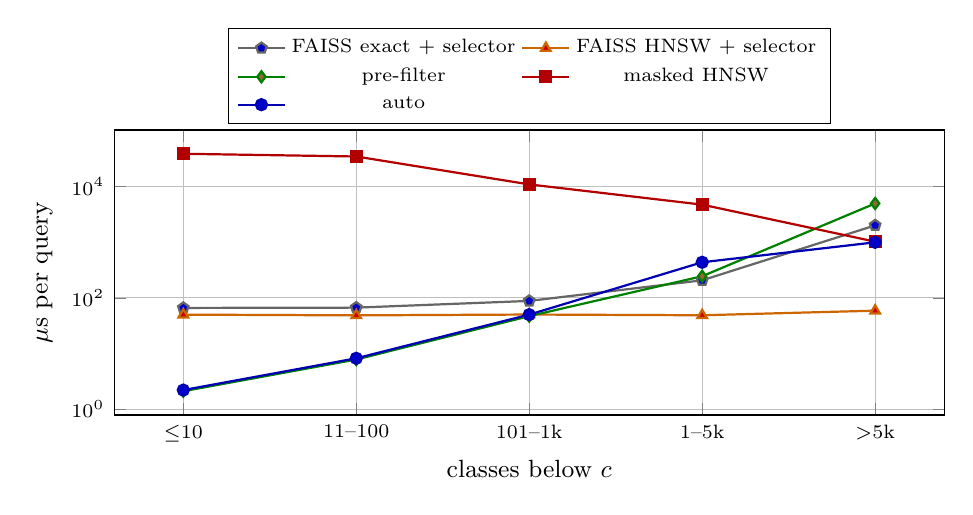
\begin{tikzpicture}
\begin{axis}[width=\columnwidth,height=5.2cm,ymode=log,symbolic x coords={<=10,11-100,101-1000,1001-5000,>5000},xtick=data,xticklabels={$\le$10,11--100,101--1k,1--5k,$>$5k},xlabel={classes below $c$},ylabel={$\mu$s per query},grid=both,legend style={font=\scriptsize,at={(0.5,1.02)},anchor=south,legend columns=2},tick label style={font=\scriptsize},label style={font=\small}]
\addplot+[mark=pentagon*,color=black!60,thick] coordinates {(<=10,66.0) (11-100,66.8) (101-1000,88.2) (1001-5000,207.0) (>5000,2011.9)};
\addlegendentry{FAISS exact + selector}
\addplot+[mark=triangle*,color=orange!80!black,thick] coordinates {(<=10,50.0) (11-100,48.5) (101-1000,50.2) (1001-5000,48.7) (>5000,58.9)};
\addlegendentry{FAISS HNSW + selector}
\addplot+[mark=diamond*,color=green!50!black,thick] coordinates {(<=10,2.1) (11-100,7.8) (101-1000,47.0) (1001-5000,244.9) (>5000,4987.1)};
\addlegendentry{pre-filter}
\addplot+[mark=square*,color=red!70!black,thick] coordinates {(<=10,38996.8) (11-100,34846.6) (101-1000,10971.5) (1001-5000,4747.7) (>5000,1025.3)};
\addlegendentry{masked HNSW}
\addplot+[mark=*,color=blue!70!black,thick] coordinates {(<=10,2.2) (11-100,8.2) (101-1000,50.0) (1001-5000,436.9) (>5000,997.7)};
\addlegendentry{auto}
\end{axis}
\end{tikzpicture}

\caption{Mean microseconds per query by number of classes below $c$, pooled over the ontologies and query kinds (log scale).}
\label{fig-latency}
\end{figure}

\stitle{Interval filtering is exact and fast where it matters}.
The auto rule returns recall 0.999, and none of its 958 queries is below 0.99; its median
is 26\,$\mu$s and its mean 206\,$\mu$s.
An exact FAISS scan with the same selector has median 60\,$\mu$s and mean 300\,$\mu$s, so
the rule is 2.3 times faster at the median and 1.5 times on average, while the approximate
indexes, which are 4 to 6 times faster than the rule on average (50 and 36\,$\mu$s), are
wrong more often than right.
The gain is largest for small classes: with at most ten members, pre-filtering takes
2.1\,$\mu$s, 33 times less than the 70\,$\mu$s of the FAISS scan, which must test a
bitmap against all $N$ rows.
From 1,001 to 5,000 members the FAISS scan is faster than pre-filtering (214 against
244\,$\mu$s inside) and than the rule (396\,$\mu$s inside, 652 outside);
above 5,000 members the rule's masked HNSW beats the exact scan for queries inside the
class (456 against 2,000\,$\mu$s) and matches it for queries outside (1.9 against 2.0\,ms).
Synonym queries, whose vectors are not stored, behave like inside queries.

\subsection{RQ3: The Rule}

Table~\ref{tab-correlation} shows the correlation: for a query inside a class of 101 to
1,000 members, 31\% of the unfiltered top 100 lie under the class, where an independent
filter would pass 1.2\% of the terms, and for a query outside it 1\%; for the largest
classes 59\% inside against 33\% expected, and 24\% outside.
The independence estimate $k/f(c)$ of the candidates a post-filter needs is therefore too
high inside and too low outside, and the post-filtering strategies show it: post-filtered
HNSW takes 34.5\,ms on average because it must widen until it finds $k$ allowed rows, and
post-filtered IVF has recall 0.61 because it stops widening too soon.

\begin{table}[t]
\caption{Masked HNSW with the filter tested per row against the class's intervals, and with the filter resolved first into a bitmap by range scans (resolving is timed): microseconds per query, pooled over the ontologies.}
\label{tab-resolve}
\small
\begin{tabular}{@{}lrrr@{}}
\toprule
Below $c$ & interval test & resolve, then bitmap & ratio \\
\midrule
$\le$10 & 42.2\,k & 41.1\,k & 1.0$\times$ \\
11--100 & 38.1\,k & 37.4\,k & 1.0$\times$ \\
101--1,000 & 12.0\,k & 11.9\,k & 1.0$\times$ \\
1,001--5,000 & 5.3\,k & 5.4\,k & 1.0$\times$ \\
$>$5,000 & 1.2\,k & 3.3\,k & 2.7$\times$ \\
\bottomrule
\end{tabular}
\end{table}


\noindent
Testing the filter per row costs the same as resolving it into a bitmap up to 5,000
members (Table~\ref{tab-resolve}) and 2.7 times less above, where resolving takes more
time than the walk it serves.
The cost model of Section~\ref{sec-filter} predicts the crossover: the mean pre-filter
cost per member is $\gamma_m=0.15\,\mu$s (median 0.11), and the masked walk over classes of
more than 5,000 members takes $\gamma_h=506\,\mu$s for queries inside, 615 for synonyms, and
1,942 for outside queries, so $\theta=\gamma_h/\gamma_m$ is about 3,400 to 13,000.

\begin{table}[t]
\caption{The auto rule at other thresholds: mean microseconds per query over every class size and query kind (all strategies return recall at least 0.99 except as noted).}
\label{tab-threshold}
\small
\begin{tabular}{@{}lrrrr@{}}
\toprule
Threshold & GO & HPO & Uberon & ChEBI \\
\midrule
256 & 609 & 246 & 301 & 6.9\,k \\
1,024 & 456 & 169 & 71 & 3.2\,k \\
4,096 & \cellcolor{ours}\textbf{111} & \cellcolor{ours}\textbf{59} & \cellcolor{ours}\textbf{41} & 533 \\
16,384 & 148 & 62 & 79 & \cellcolor{ours}\textbf{426} \\
65,536 & 180 & 114 & 79 & 567 \\
\bottomrule
\end{tabular}
\end{table}


\begin{table}[t]
\caption{A second embedding model, \texttt{all-mpnet-base-v2} (768 dimensions): recall@10 / mean microseconds over every class size and query kind, and the share of the unfiltered top 100 under the class for queries inside and outside.}
\label{tab-model}
\small
\resizebox{\columnwidth}{!}{%
\begin{tabular}{@{}lrrrrrr@{}}
\toprule
Ontology & FAISS IVF & FAISS HNSW & pre-filter & auto & top-100 under $c$, inside & outside \\
\midrule
GO & 0.64 / 51 & 0.67 / 81 & 1.00 / 279 & 1.00 / 195 & 0.30 & 0.02 \\
HPO & 0.68 / 43 & 0.71 / 77 & 1.00 / 181 & 1.00 / 94 & 0.37 & 0.05 \\
\bottomrule
\end{tabular}}
\end{table}


\noindent
Table~\ref{tab-threshold} confirms it: a threshold of 4,096 is best on the Gene Ontology,
the Human Phenotype Ontology, and Uberon, and 16,384 on ChEBI, whose walks are costlier;
256 and 1,024 are 1.7 to 7 times slower than the best, and 65,536 is 1.3 to 1.9 times
slower.
A single threshold of 4,096 is within 25\% of the best on all four.

\stitle{The number of neighbors}.
Table~\ref{tab-k} varies $k$ on the Gene Ontology: asking for one neighbor or fifty changes
the approximate indexes' recall by at most 0.1 (0.70 to 0.55 for IVF), and the rule stays
exact, at a mean of 107 to 115\,$\mu$s.

\begin{table}[t]
\caption{The number of neighbors asked for, on the Gene Ontology: recall / mean microseconds over every class size and query kind.}
\label{tab-k}
\small
\begin{tabular}{@{}lrrrr@{}}
\toprule
$k$ & FAISS IVF & FAISS HNSW & pre-filter & auto \\
\midrule
1 & 0.70 / 31 & 0.75 / 46 & 1.00 / 173 & 1.00 / 107 \\
10 & 0.63 / 31 & 0.67 / 47 & 1.00 / 178 & 1.00 / 110 \\
50 & 0.55 / 33 & 0.56 / 49 & 1.00 / 182 & 1.00 / 115 \\
\bottomrule
\end{tabular}
\end{table}


\stitle{Another embedding model}.
Table~\ref{tab-model} repeats the study on the Gene Ontology and the Human Phenotype
Ontology with \texttt{all-mpnet-base-v2}, a larger model with 768 dimensions, and the picture
holds: FAISS's IVF and HNSW return recall 0.64 to 0.71, the rule returns 1.00, and the
correlation is as strong (0.30 and 0.37 of the unfiltered top 100 under the class for inside
queries, 0.02 and 0.05 for outside).

\stitle{Threats to validity}.
The members FAISS filters with come from a table built outside the timer, which favors it;
FAISS and DuckDB are called from Python, whose per-call overhead (about 10\,$\mu$s) matters
for the 2\,$\mu$s queries; each index is built once, so HNSW's randomness is one draw;
the ontologies are four of the OBO Foundry's, with names embedded by two sentence models,
and the queries are sampled by class size, not by use.
The comparison with FAISS's approximate indexes is one of default-style settings and of a
wide budget, not of tuned ones.

\subsection{RQ4: The Indexes}

\begin{table*}[t]
\caption{Unfiltered ten-nearest-neighbor search, 1,000 queries: recall@10 / microseconds per query. FAISS is called once per query from Python, like \sys{} (its call overhead, about 10\,$\mu$s, is included); batched numbers are in the appendix. IVF: nprobe 16; HNSW: $M{=}16$, $\mathit{ef}{=}40$. Build seconds in parentheses.}
\label{tab-index}
\small
\begin{tabular}{@{}lccccccc@{}}
\toprule
Ontology & terms & flat (\sys{}) & flat (FAISS) & IVF (\sys{}) & IVF (FAISS) & HNSW (\sys{}) & HNSW (FAISS) \\
\midrule
GO & 38,092 & 1.00 / 2.2\,k & 1.00 / 1.1\,k & 0.93 / 289 (18\,s) & 0.93 / 71 & 1.00 / 123 (16\,s) & 1.00 / 58 \\
HPO & 19,894 & 1.00 / 1.2\,k & 1.00 / 610 & 0.93 / 222 (8\,s) & 0.92 / 50 & 1.00 / 190 (9\,s) & 1.00 / 45 \\
Uberon & 15,047 & 1.00 / 907 & 1.00 / 432 & 0.91 / 142 (5\,s) & 0.91 / 50 & 1.00 / 77 (6\,s) & 1.00 / 39 \\
ChEBI & 218,723 & 1.00 / 13.1\,k & 1.00 / 6.6\,k & 0.93 / 1.1\,k (115\,s) & 0.92 / 295 & 0.99 / 169 (142\,s) & 0.98 / 201 \\
\bottomrule
\end{tabular}
\end{table*}


\noindent
Table~\ref{tab-index} compares the indexes unfiltered.
Called one query at a time, \sys's exact scan is 2.0 times slower than FAISS's, its IVF
2.8 to 4.4 times slower, and its HNSW 2.0 to 4.2 times slower on the three smaller
ontologies and 0.8 times (faster) on ChEBI; recalls match to within 0.01.
The IVF gap is the price of the design: each list entry is a decoded 24-byte key and a
random read of the vector, about 2.7 times the cost per scored row of a contiguous list,
bought in exchange for lists that page, cache, and latch with the triples and need no
second copy of the data.
Building is slower too (IVF 115\,s and HNSW 142\,s on ChEBI against 5 and 83\,s).
Batching favors FAISS further, since its flat scan becomes a matrix product (Appendix,
Table~\ref{tab-index-batched}).
On ChEBI, 218,723 terms and 320\,MiB of vectors, the rule still returns recall 0.99 or
more on every query, with a mean of 543\,$\mu$s (FAISS's exact scan: 846\,$\mu$s).

\begin{table}[t]
\caption{Filtered queries per second on one to eight threads over the whole workload: the auto rule (C++ threads, one shared index) against FAISS's exact scan and HNSW with an ID selector (Python threads; FAISS releases the interpreter lock while it searches).}
\label{tab-scale}
\small
\resizebox{\columnwidth}{!}{%
\begin{tabular}{@{}lrrrrrr@{}}
\toprule
 & \multicolumn{2}{c}{auto} & \multicolumn{2}{c}{FAISS exact} & \multicolumn{2}{c}{FAISS HNSW} \\
\cmidrule(lr){2-3}\cmidrule(lr){4-5}\cmidrule(lr){6-7}
Ontology & 1 & 8 & 1 & 8 & 1 & 8 \\
\midrule
GO & 6,144 & 31k & 9,106 & 42k & 11k & 43k \\
HPO & 15k & 88k & 17k & 46k & 15k & 40k \\
Uberon & 21k & 119k & 21k & 51k & 17k & 40k \\
ChEBI & 1,327 & 7,576 & 1,085 & 5,091 & 7,001 & 35k \\
\bottomrule
\end{tabular}}
\end{table}


\noindent
On eight threads (Table~\ref{tab-scale}) the rule scales 5.0 to 5.9 times on every ontology,
because its search shares only the read-only index and the engine's latch-free buffer pool;
FAISS's exact scan scales 2.4 to 4.7 times through Python threads.
At eight threads the rule serves 1.9, 2.3, and 1.5 times the queries of FAISS's exact
scan on HPO, Uberon, and ChEBI, and 0.7 times on the Gene Ontology, where the exact
scan is faster at one thread as well.

\section{Related Work}
\label{sec-related}

\stitle{Vector search}.
Approximate nearest neighbor search has inverted files and product
quantization~\cite{jegou2011}, proximity graphs such as HNSW~\cite{malkov2020}, and
disk-oriented graphs such as DiskANN~\cite{subramanya2019}; FAISS~\cite{johnson2021,douze2024}
and hnswlib implement them, and vector database systems such as Milvus~\cite{wang2021milvus}
wrap them with storage and a query language; Pan, Wang, and Li survey the hybrid
queries, an attribute predicate plus a vector, that are hard for them~\cite{pan2024}.

\stitle{Filtered search}.
Filtered-DiskANN builds a graph whose edges respect label filters~\cite{gollapudi2023},
and ACORN makes HNSW traverse only the nodes that pass a predicate and densifies the
graph so that it stays connected~\cite{patel2024}.
Both treat the filter as an opaque attribute of the vector; a class filter is not
opaque, because the hierarchy supplies a structure that makes membership a binary search
and the filter correlated with the vectors, which is what we measure and use.
FAISS's ID selectors, the baseline here, pass a predicate to the index's own search.

\stitle{Hierarchies in stores}.
Agrawal, Borgida, and Jagadish~\cite{agrawal1989} label a hierarchy with postorder
intervals, and Grust~\cite{grust2002} numbers XML trees; RDFS entailment is otherwise
rewritten or materialized~\cite{rdfox}.
Neo4j, Neptune Analytics, Fluree, and GraphDB add vector or similarity indexes to graph
and RDF stores~\cite{neo4jvec,neptunevec,fluree,graphdbsim}; in the documentation we
read, none restricts the search with range-scannable hierarchy intervals in the engine
that holds the triples.
Embeddings of the hierarchy itself, such as hyperbolic embeddings~\cite{nickel2017}, would
change the vectors, not the filter.

\stitle{Order and similarity}.
Space-filling curves and sorting keys map points to one dimension and keep neighbors
close on average; the bandwidth argument says they cannot keep all of them close, and the
adaptive radix tree~\cite{leis2013} orders keys by byte and falls under the same bound.

\section{Conclusion}
\label{sec-conclude}

An ontology's hierarchy is a better filter for vector search than an attribute the
index cannot see.
Postorder intervals in the store's B+ tree make a class's members a few range scans and
membership a binary search; a vector search can then test the filter per row, or
resolve it and score the members exactly, and a cost model with one threshold picks the
cheaper.
On four ontologies this answers $\mathrm{near}(q,c,k)$ with recall 0.999 and a median of
26\,$\mu$s, where FAISS indexes with ID selectors return recall 0.61 and 0.64 and lose
almost every answer for a query outside a small class, and where an exact FAISS scan is
33 times slower for classes of at most ten members.
No sorted order of the terms can do the same: every order separates some neighbors by
$(N{-}1)/D$ positions, and the best we found holds at most 56\% of a term's neighbors in
a window of 200.

\stitle{Limitations}.
Our IVF and HNSW are 2 to 4 times slower than FAISS's when called one query at a time and
take longer to build, the price of keeping lists in the triple tree; the vectors are held
in memory and the indexes are rebuilt, not updated, when they change; the labels are
rebuilt when the hierarchy changes; the embeddings come from one small model that
embeds names only; masked HNSW is slow for classes of a few hundred members and under,
which the rule avoids and a denser graph, as ACORN builds~\cite{patel2024}, might fix;
and for classes of 1,001 to 5,000 members an exact FAISS scan with a precomputed member
bitmap is faster than our rule.


\bibliographystyle{ACM-Reference-Format}
\bibliography{refs}

\clearpage
\appendix
\section*{Appendix}
\section{Proofs}
\label{apx-proofs}

\begin{proof}[Proof of Lemma~\ref{lem-bw}]
The first and last vertices of the order are $N-1$ apart and joined by a path of at most
$D$ edges, so some edge of the path covers at least $(N-1)/D$ positions.
\end{proof}

\begin{proof}[Proof of Lemma~\ref{lem-exact}]
Pre-filter scores every member of $\desc(c)$ and keeps the $k$ best, which is
$\mathrm{near}(q,c,k)$ by definition.
Masked IVF scores only rows whose number lies in an interval of $I(c)$, which are the
members; it stops when it holds $k$ of them after $\rho$ lists, or after all $\nu$ lists,
so it returns $k$ members if $|\desc(c)|\ge k$ and all otherwise.
With $\rho=\nu$ it has scored every member and keeps the $k$ best, which is
$\mathrm{near}(q,c,k)$.
\end{proof}

\section{More Measurements}
\label{apx-more}

\begin{table}[t]
\caption{Per ontology, over every class size and query kind: recall@10, and mean / median microseconds per query.}
\label{tab-per-ontology}
\small
\resizebox{\columnwidth}{!}{%
\begin{tabular}{@{}lrrrrr@{}}
\toprule
Ontology & queries & auto & FAISS flat & FAISS IVF & FAISS HNSW \\
\midrule
GO & 247 & 1.00 / 110 / 26 & 1.00 / 117 / 46 & 0.63 / 31 / 27 & 0.67 / 47 / 47 \\
HPO & 237 & 1.00 / 59 / 18 & 1.00 / 66 / 29 & 0.67 / 27 / 23 & 0.72 / 45 / 46 \\
Uberon & 201 & 1.00 / 41 / 8.3 & 1.00 / 57 / 22 & 0.62 / 23 / 20 & 0.67 / 43 / 43 \\
ChEBI & 273 & 1.00 / 543 / 59 & 1.00 / 846 / 224 & 0.55 / 59 / 50 & 0.54 / 63 / 65 \\
\bottomrule
\end{tabular}}
\end{table}


\begin{table*}[t]
\caption{Unfiltered search with FAISS and hnswlib answering the 1,000 queries in one batch on one thread: recall@10 / microseconds per query. The flat scan is a matrix product, which one-query-at-a-time search cannot use.}
\label{tab-index-batched}
\small
\begin{tabular}{@{}lccccc@{}}
\toprule
Ontology & flat & IVF (nprobe 16) & HNSW ($\mathit{ef}{=}40$), FAISS & HNSW ($\mathit{ef}{=}40$), hnswlib & IVF (nprobe 64) \\
\midrule
GO & 1.00 / 30 & 0.93 / 60 & 1.00 / 58 & 1.00 / 250 & 0.98 / 192 \\
HPO & 1.00 / 17 & 0.92 / 38 & 1.00 / 44 & 1.00 / 256 & 0.97 / 132 \\
Uberon & 1.00 / 13 & 0.91 / 35 & 1.00 / 36 & 1.00 / 241 & 0.97 / 120 \\
ChEBI & 1.00 / 162 & 0.92 / 124 & 0.98 / 91 & 0.98 / 299 & 0.96 / 447 \\
\bottomrule
\end{tabular}
\end{table*}



\end{document}
